%%%%%%%%%%%%%%%%%%%%%%%%%%%%%%%%%%%%%%%%%%%%%%%%%%%%%%%%%%%%%%%%%%%%%
% Mitschrieb vom 09.01.2014                                         %
%%%%%%%%%%%%%%%%%%%%%%%%%%%%%%%%%%%%%%%%%%%%%%%%%%%%%%%%%%%%%%%%%%%%%
\chapter{Euklidische und Nichteuklidische Geometrie}
\section{Axiome für die euklidische Ebene}
Axiome\xindex{Axiom} bilden die Grundbausteine jeder mathematischen Theorie. Eine
Sammlung aus Axiomen nennt man Axiomensystem\xindex{Axiomensystem}.
Da der Begriff des Axiomensystems so grundlegend ist, hat man auch 
ein paar sehr grundlegende Forderungen an ihn: Axiomensysteme sollen
\textbf{widerspruchsfrei} sein, die Axiome sollen möglichst
\textbf{unabhängig} sein und \textbf{Vollständigkeit} wäre auch toll.
Mit Unabhängigkeit ist gemeint, dass kein Axiom sich aus einem anderem
herleiten lässt. Dies scheint auf den ersten Blick eine einfache
Eigenschaft zu sein. Auf den zweiten Blick muss man jedoch einsehen, 
dass das Parallelenproblem, also die Frage ob das Parallelenaxiom 
unabhängig von den restlichen Axiomen ist, über 2000 Jahre nicht 
gelöst wurde. Ein ganz anderes Kaliber ist die Frage nach der
Vollständigkeit. Ein Axiomensystem gilt als Vollständig, wenn
jede Aussage innerhalb des Systems verifizierbar oder falsifizierbar
ist. Interessant ist hierbei der Gödelsche Unvollständigkeitssatz, 
der z.~B. für die Arithmetik beweist, dass nicht alle Aussagen
formal bewiesen oder widerlegt werden können.

Kehren wir nun jedoch zurück zur Geometrie. Euklid hat in seiner 
Abhandlung \enquote{Die Elemente} ein Axiomensystem für die Geometrie
aufgestellt. 

\textbf{Euklids Axiome}
\begin{itemize}
    \item \textbf{Strecke} zwischen je zwei Punkten
    \item Jede Strecke bestimmt genau eine \textbf{Gerade}
    \item \textbf{Kreis} (um jeden Punkt mit jedem Radius)
    \item Je zwei rechte Winkel sind gleich (Isometrie, Bewegung)
    \item Parallelenaxiom: Euklid:\\
        Wird eine Gerade so von zwei Geraden geschnitten, dass die 
        Summe der Innenwinkel zwei Rechte ist, dann schneiden sich
        diese Geraden auf der Seite dieser Winkel.\\
        \\
        Man mache sich klar, dass das nur dann nicht der Fall ist, 
        wenn beide Geraden parallel sind und senkrecht auf die erste stehen.
\end{itemize}

\begin{definition}\xindex{Ebene!euklidische}%In Vorlesung: Definition 14.2
    Eine \textbf{euklidische Ebene} ist ein metrischer Raum $(X,d)$ 
    zusammen mit einer Teilmenge $G \subseteq \powerset{X}$, sodass die
    Axiome~\ref{axiom:1}~-~\ref{axiom:4} erfüllt sind:
    \begin{enumerate}[label=§\arabic*),ref=§\arabic*]
        \item \textbf{Inzidenzaxiome}:\label{axiom:1}
            \begin{enumerate}[label=(\roman*),ref=\theenumi{} (\roman*)]
                \item Zu $P \neq Q \in X$ gibt es genau ein $g \in G$ mit
                      $\Set{P, Q} \subseteq g$.
                \item $|g| \geq 2 \;\;\; \forall g \in G$
                \item $X \in G$
            \end{enumerate}
        \item \textbf{Abstandsaxiom}: Zu $P, Q, R \in X$ gibt es \label{axiom:2}
              genau dann ein $g \in G$ mit $\Set{P, Q, R} \subseteq g$,
              wenn gilt: 
              \begin{itemize}[]
                \item $d(P, R) = d(P, Q) + d(Q, R)$ oder
                \item $d(P, Q) = d(P, R) + d(R, Q)$ oder
                \item $d(Q, R) = d(Q, P) + d(P, R)$
              \end{itemize}
    \end{enumerate}
\end{definition}

\begin{definition}
    \begin{enumerate}[label=\alph*)]
        \item $P, Q, R$ liegen \textbf{kollinear}\xindex{kollinear}, 
              wenn es $g \in G$ gibt mit $\Set{P, Q, R} \subseteq g$.
        \item $Q$ \textbf{liegt zwischen}\xindex{liegt zwischen} $P$
              und $R$, wenn $d(P, R) = d(P, Q) + d(Q, R)$
        \item \textbf{Strecke}\xindex{Strecke} $\overline{PR} := \Set{Q \in X | Q \text{ liegt zwischen } P \text{ und } R}$
        \item \textbf{Halbgeraden}\xindex{Halbgerade}:\\
              $PR^+ := \Set{Q \in X | Q \text{ liegt zwischen } P \text{ und } R \text{ oder } R \text{ liegt zwischen } P \text{ und } Q}$\\
              $PR^- := \Set{Q \in X | P \text{ liegt zwischen } Q \text{ und } R}$\\ 
    \end{enumerate}
\end{definition}

\begin{figure}[htp]
    \centering
    \documentclass[varwidth=true, border=2pt]{standalone}
\usepackage{tikz}
\usetikzlibrary{snakes}

\begin{document}
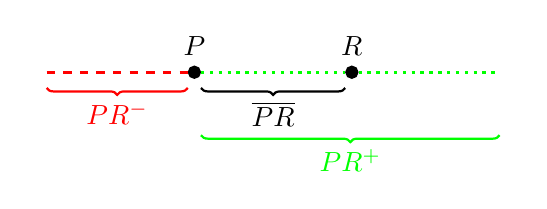
\begin{tikzpicture}
    \tikzstyle{point}=[circle,thick,draw=black,fill=black,inner sep=0pt,minimum width=4pt,minimum height=4pt]
    \node (Pleft) at (0,0) {};
    \node (P)[point,label=90:$P$] at (2,0) {};
    \node (R)[point,label=90:$R$] at (4,0) {};
    \node (Rright) at (6,0) {};
    \draw[red,dashed,very thick] (Pleft) -- (P);
    \draw[green,dotted,very thick] (P) -- (R) -- (Rright);
    \draw [thick,decoration={brace,mirror,raise=0.2cm},decorate,red] (Pleft) -- (P) node [pos=0.5,anchor=north,yshift=-0.25cm,red] {$PR^-$}; 
    \draw [thick,decoration={brace,mirror,raise=0.2cm},decorate] (P) -- (R) node [pos=0.5,anchor=north,yshift=-0.25cm] {$\overline{PR}$}; 
    \draw [thick,decoration={brace,mirror,raise=0.8cm},decorate,green] (P) -- (Rright) node [pos=0.5,anchor=north,yshift=-0.85cm,green] {$PR^+$}; 
\end{tikzpicture}
\end{document}

    \caption{Halbgeraden}
    \label{fig:halbgeraden}
\end{figure}

\begin{korollar}
    \begin{enumerate}[label=(\roman*)]
        \item $PR^+ \cup PR^- = PR$
        \item $PR^+ \cap PR^- = \Set{P}$
    \end{enumerate}
\end{korollar}

\begin{beweis}\leavevmode
    \begin{enumerate}[label=(\roman*)]
        \item \enquote{$\subseteq$} folgt direkt aus der Definition von $PR^+$ und $PR^-$\\
              \enquote{$\supseteq$}: Sei $Q \in PR \Rightarrow P, Q, R$ 
              sind kollinear.\\
              $\stackrel{\ref{axiom:2}}{\Rightarrow}
              \begin{cases} 
                Q \text{ liegt zwischen } P \text{ und } R \Rightarrow Q \in PR\\
                R \text{ liegt zwischen } P \text{ und } Q \Rightarrow Q \in PR\\
                P \text{ liegt zwischen } Q \text{ und } R \Rightarrow Q \in PR
              \end{cases}$
        \item \enquote{$\supseteq$} ist offensichtlich\\
              \enquote{$\subseteq$}: Sei $PR^+ \cap PR^-$. Dann ist
              $d(Q,R) = d(P,Q) + d(P,R)$ weil $Q \in PR^-$ und
              \begin{align*}
                &\left \{ \begin{array}{l}
                        d(P,R) = d(P,Q) + d(Q,R) \text{ oder }\\
                        d(P,Q) = d(P,R) + d(R,Q)
                       \end{array} \right \}\\
                &\Rightarrow d(Q,R) = 2d(P,Q) + d(Q,R)\\
                &\Rightarrow d(P,Q) = 0\\
                &\Rightarrow P=Q\\
                &d(P,Q) = 2d(P,R) + d(P,Q)\\
                &\Rightarrow P=R\\
                &\Rightarrow \text{Widerspruch}
              \end{align*}
    \end{enumerate}
\end{beweis}

\begin{definition}
    \begin{enumerate}[label=§\arabic*),ref=§\arabic*,start=3]
        \item \textbf{Anordnungsaxiome}\label{axiom:3}
            \begin{enumerate}[label=(\roman*),ref=§\theenumi{} (\roman*)]
                \item  Zu jedem $P \in X$ jeder Halbgerade $H$ mit \label{axiom:3.1}
                      Anfangspunkt $P$ und jedem $r \in \mdr_{\geq 0}$
                      gibt es genau ein $Q \in H$ mit $d(P,Q) = r$.
                \item Jede Gerade zerlegt $X \setminus g = H_1 \dcup H_2$
                      in zwei nichtleere Teilmengen $H_1, H_2$.
                      (Diese Teilmengen heißen \textbf{Halbebenen}\xindex{Halbebene} bzgl. $g$),
                      sodass für alle $A \in H_i$, $B \in H_j$
                      $(i,j \in \Set{1,2})$ gilt: $\overline{AB} \cap g \neq \emptyset \Leftrightarrow i \neq j$\label{axiom:3.2}
            \end{enumerate}
        \item \textbf{Bewegungsaxiome}: Zu $P, Q, P', Q' \in X$\label{axiom:4}
            mit $d(P,Q) = d(P', Q')$. Isometrien $\varphi_1, \varphi_2$
            mit $\varphi_i (P) = P'$ und $\varpi_i(Q) = Q', i=1,2$
            (Spiegelung an der Gerade durch $P$ und $Q$ ist nach 
             Identifizierung von $P \cong P'$ und $Q \cong Q'$ eine
             weitere Isometrie.)
        \item \textbf{Parallelenaxiom}: Für jedes $g \in G$ und jedes
            $P \in X \setminus g$ gibt es höchstens ein $k \in G$ mit
            $h \cap g = \emptyset$.\footnote{$h$ heißt \enquote{Parallele zu $g$ durch $P$}.}
    \end{enumerate}
\end{definition}

\todo[inline]{Bilder zu Parallelenaxiom, Inzidenzaxiom und Bewegungsaxiom}

%%%%%%%%%%%%%%%%%%%%%%%%%%%%%%%%%%%%%%%%%%%%%%%%%%%%%%%%%%%%%%%%%%%%%
% Mitschrieb vom 14.01.2014                                         %
%%%%%%%%%%%%%%%%%%%%%%%%%%%%%%%%%%%%%%%%%%%%%%%%%%%%%%%%%%%%%%%%%%%%%

\begin{satz}[Satz von Rasch]\label{satz:rasch} %In Vorlesung: Bemerkung 14.5
    Seien $P$, $Q$, $R$ nicht kollinear, $g \in G$ mit $g \cap \Set{P, Q, R} = \emptyset$
    und $g \cap \overline{PQ} \neq \emptyset$. Dann ist
    $g \cap \overline{PR} \neq \emptyset$ oder $g \cap \overline{QR} \neq \emptyset$.
\end{satz}

\begin{beweis}
    $g \cap \overline{PQ} \neq \emptyset \stackrel{\ref{axiom:3.2}}{\Rightarrow}$
    $P$ und $Q$ liegen in verschiedenen Halbebenen bzgl. $g$
    $\Rightarrow$ \obda $R$ und $P$ liegen in verschieden
    Halbebenen bzgl. $P$.
    $\Rightarrow g \cap \overline{RP} \neq \emptyset$
\end{beweis}

\begin{proposition}%In Vorlesung: Satz 14.4
    In einer Geometrie, die \ref{axiom:1}~-~\ref{axiom:3} erfüllt,
    gibt es zu $P, P', Q, Q'$ mit $d(P, Q) = d(P', Q')$ höchstens
    zwei Isometrien mit $\varphi(P) = P'$ und $\varphi(Q) = Q'$

    Aus den Axiomen  folgt, dass es in 
    den Situation \ref{axiom:4} höchstens zwei Isometrien mit
    $\varphi_i(P) = P'$ und $\varphi_i(Q) = Q'$ gibt.
\end{proposition}

\begin{beweis}
    Seien $\varphi_1, \varphi_2, \varphi_3$ Isometrien mit
    $\varphi_i(P) = P'$, $\varphi_i(Q) = Q'$, $i=1,2,3$

    \begin{behauptung}[1]
        $\exists R \in X \setminus PQ$ mit $\varphi_{1} (R) = \varphi_{2} (R)$.
    \end{behauptung}
    \begin{behauptung}[2]
        Hat $\varphi$ 3 Fixpunkte, die nicht kollinear sind,
        so ist $\varphi = \id_X$.
    \end{behauptung}

    \begin{behauptung}[2']
        $(\varphi(P) = P \land \varphi(Q) = Q) \Rightarrow (\varphi(S) = S\;\forall S \in PQ)$
    \end{behauptung}

    Aus Beh. 1 und Beh. 2 folgt, dass $\varphi_2^{-1} \circ \varphi_1 = \id_X$,
    also $\varphi_2 = \varphi_1$.

    \begin{beweis}\leavevmode
        \begin{behauptung}
            Sind $P \neq Q$ Fixpunkte einer Isometrie, so ist 
            $\varphi(R) = R$ für jedes $R \in PQ$.
        \end{behauptung}
        \begin{beweis}
            Seien $P$, $Q$ und $R$ Fixpunkte von $\varphi$, $R \in PG$
            und $A \notin \overline{PQ} \cup \overline{PR} \cup \overline{QR}$.
            Sei $B \in \overline{PQ} \setminus \Set{P, Q}$. Dann ist
            $\varphi(B) = B$ wegen Beh.~2'.

            Ist $R \in AB$, so enthält $AB$ 2 Fixpunkte von $\varphi$
            $\stackrel{Beh.~2'}{\Rightarrow} \varphi(A) = A$.

            \begin{figure}[htp]
                \centering
                \documentclass[varwidth=true, border=2pt]{standalone}
\usepackage{tikz}

\begin{document}
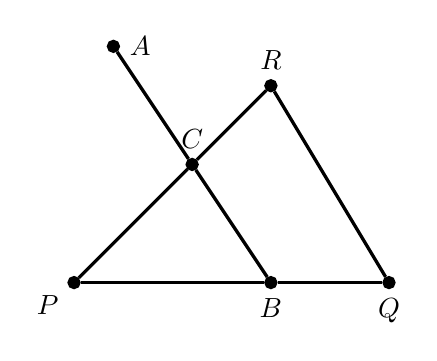
\begin{tikzpicture}
    \tikzstyle{point}=[circle,thick,draw=black,fill=black,inner sep=0pt,minimum width=4pt,minimum height=4pt]
    \node (P)[point,label={[label distance=0cm]210:$P$}] at (0,0) {};
    \node (B)[point,label={[label distance=0cm]-90:$B$}] at (2.5,0) {};
    \node (Q)[point,label={[label distance=0cm]-90:$Q$}] at (4,0) {};
    \node (C)[point,label={[label distance=0cm]90:$C$}] at (1.5,1.5) {};
    \node (R)[point,label={[label distance=0cm]90:$R$}] at (2.5,2.5) {};

    \node (A)[point,label={[label distance=0cm]0:$A$}] at (0.5,3) {};

    \draw[very thick] (P) edge node  {} (B);
    \draw[very thick] (B) edge node  {} (Q);
    \draw[very thick] (P) edge node  {} (C);
    \draw[very thick] (C) edge node  {} (R);

    \draw[very thick] (B) edge node  {} (C);
    \draw[very thick] (C) edge node  {} (A);

    \draw[very thick] (Q) edge node  {} (R);
\end{tikzpicture}
\end{document}

                \caption{$P, Q, R$ sind Fixpunke, $B \in \overline{PQ} \setminus \Set{P,Q}$, $A \notin PQ \cup PR \cup QR$}
                \label{fig:geometry-1}
            \end{figure}

            Ist $R \notin AB$, so ist $AB \cap \overline{PR} \neq \emptyset$
            oder $AB \in \overline{RQ} \neq \emptyset$ nach \cref{satz:rasch}.
            Der Schnittpunkt $C$ ist dann Fixpunkt von $\varphi'$
            nach Beh.~2' $\Rightarrow \varphi(A) = A$.
        \end{beweis}

        \begin{beweis}[Beweis 1]
            Sei $R \in X \setminus PQ$. Von den drei Punkten 
            $\varphi_1(R), \varphi_2(R), \varphi_3(R)$ liegen zwei
            in der selben Halbebene bzgl. $P'Q' = \varphi_i(PQ)$.

            \Obda seien $\varphi_1(R)$ und $\varphi_2(R)$ in der 
            selben Halbebene.

            Es gilt: 
            \begin{align}
                d(P', \varphi_1(R)) &= d(\varphi_1(P), \varphi_1(R))\\
                    &= d(P, R)\\
                    &= d(\varphi_2(P), \varphi_2(R))\\
                    &= d(P', \varphi_2(R))\\
                    &= d(Q', \varphi_2(R))
            \end{align}
            und analog $d(Q', \varphi_1(R)) = d(Q', \varphi_2(R))$

            \begin{figure}[htp]
                \centering
                \begin{tikzpicture}
    \tikzstyle{point}=[circle,thick,draw=black,fill=black,inner sep=0pt,minimum width=4pt,minimum height=4pt]
    \node (P)[point,label={[label distance=0cm]-90:$P$}] at (0,0) {};
    \node (Q)[point,label={[label distance=0cm]-90:$Q$}] at (5,1) {};
    \node (A)[point,label={[label distance=0cm]180:$A$}] at (2,2) {};
    \node (B)[point,label={[label distance=0cm]190:$B$}] at (1,3) {};

    \draw[very thick] (P) edge node  {} (Q);
    \draw[very thick, red] (P) edge node {} (A);
    \draw[very thick, red] (P) edge node {} (B);
    \draw[very thick, blue] (Q) edge node {} (A);
    \draw[very thick, blue] (Q) edge node {} (B);

    \draw[very thick] ($(P)!-1cm!(Q)$) -- ($(Q)!-1cm!(P)$);
\end{tikzpicture}

                \caption{Die beiden roten und die beiden blauen Linien sind gleich lang. Intuitiv weiß man, dass daraus folgt, dass $\varphi_1(R) = \varphi_2(R)$ gilt.}.
                \label{fig:bild-2}
            \end{figure}
        \end{beweis}

        \begin{korollar}\label{kor:14.6}%In Vorlesung: Bemerkung 14.6
            Seien $P, Q \in X$, $P \neq Q$, $A, B \in X \setminus PQ$
            in der selben Halbebene bzgl. $PQ$ mit $d(A, P) = d(B, P)$
            und $d(A, Q) = d(B, Q)$. Dann ist $A = B$.
        \end{korollar}
        \begin{beweis} durch Widerspruch\\
            \underline{Annahme}: $A \neq B$

            Dann ist $B \notin (PA \cup QA)$ wegen \ref{axiom:2}.

            \underline{1. Fall}: $Q$ und $B$ liegen in derselben Halbebene bzgl. $PA$
            \begin{behauptung}[Beh. 3]
                Dann ist $PB^+ \cap \overline{AQ} \neq \emptyset$
            \end{behauptung}

            \begin{figure}[htp]
                \centering
                \begin{tikzpicture}
    \tkzSetUpPoint[shape=circle,size=10,color=black,fill=black]
    \tkzSetUpLine[line width=1]
    \tkzDefPoints{0/0/P, 4/0/Q, 1/0.5/B, 1/2/A}
    \tkzInterLL(P,B)(Q,A) \tkzGetPoint{C}

    \tkzDrawLine(P,A)
    \tkzDrawLine(Q,A)
    \tkzDrawLine(P,Q)
    \tkzDrawLine[add=0 and 0.5](P,C)
    \tkzDrawSegments(B,Q)

    \tkzDrawPoints(P,Q,B,C,A)
    \tkzLabelPoint[below](P){$P$}
    \tkzLabelPoint[below](Q){$Q$}
    \tkzLabelPoint[below](B){$B$}
    \tkzLabelPoint[below](C){$C$}
    \tkzLabelPoint[below](A){$A$}
\end{tikzpicture}

                \caption{1. Fall}
                \label{fig:bild-3}
            \end{figure}

            Sei $C$ der Schnittpunkt.

            Dann gilt:
            \begin{enumerate}[label=(\roman*)]
                \item $d(A, C) + d(A, Q) = d(B, Q) < d(B, C) + d(C, Q) \Rightarrow d(A, C) < d(B, C)$ \label{enum:komischer-beweis-i}
                \item \begin{enumerate}[label=\alph*)]
                        \item $B$ liegt zwischen $P$ und $C$.

                              $d(P,A) + d(A, C) > d(P,C) = d(P,B) + d(B,c) = d(P,A) + d(B,C)$
                              $\Rightarrow d(A,c) > d(B,C) \Rightarrow$ Widerspruch zu \ref{enum:komischer-beweis-i}
                        \item $C$ liegt zwischen $P$ und $B$

                              $d(P,C) + d(C,A) > d(P,A) = d(P,B) = d(P,C) + d(C, B)$\\
                              $\Rightarrow d(C, A) > d(C, B)$\\
                              $\Rightarrow$ Widerspruch zu \ref{enum:komischer-beweis-i}
                    \end{enumerate}
            \end{enumerate}

            \underline{2. Fall}: $Q$ und $B$ liegen auf verscheiden Halbebenen bzgl. $PA$.

            \begin{figure}[htp]
                \centering
                \begin{tikzpicture}
    \tkzSetUpPoint[shape=circle,size=10,color=black,fill=black]
    \tkzSetUpLine[line width=1]
    \tkzDefPoints{0/0/P, 4/1/Q, 2/3/A, 0/3/B}

    \tkzDrawSegments(P,Q Q,A A,P)
    \tkzDrawSegments[dashed](P,B B,Q)
    \tkzDrawLine(P,Q)

    \tkzDrawPoints(P,Q,A,B)
    \tkzLabelPoint[below](P){$P$}
    \tkzLabelPoint[below](Q){$Q$}
    \tkzLabelPoint[above](A){$A$}
    \tkzLabelPoint[above](B){$B$}
\end{tikzpicture}

                \caption{2. Fall}
                \label{fig:bild-4}
            \end{figure}

            Dann liegen $A$ und $Q$ in derselben Halbebene bzgl. $PB$.

            Tausche $A$ und $B \Rightarrow$  Fall 1
        \end{beweis}

        \begin{beweis}[Beweis 3]
            \begin{figure}[htp]
                \centering
                \usetkzobj{all}
\begin{tikzpicture}
    \tkzSetUpPoint[shape=circle,size=10,color=black,fill=black]
    \tkzSetUpLine[line width=1]
    \tkzDefPoints{0/0/P, 4/1/Q, 2/3/A, 5/3/B}
    \tkzInterLL(P,B)(A,Q) \tkzGetPoint{C}
    \tkzDrawPoints(P,Q,A,B,C)

    %\tkzDrawSegments(P,Q Q,A A,P)
    %\tkzDrawSegments[dashed](P,B B,Q)
    \tkzDrawLine(P,Q)
    \tkzDrawLine(P,A)
    \tkzDrawLine(A,Q)
    \tkzDrawLine(P,B)


    \tkzLabelPoint[below](P){$P$}
    \tkzLabelPoint[below](Q){$Q$}
    \tkzLabelPoint[below](A){$A$}
    \tkzLabelPoint[below](B){$B$}
    \tkzLabelPoint[above](C){$C$}
\end{tikzpicture}

                \caption{TODO}
                \label{fig:bild-5}
            \end{figure}

            Sei $P' \in PQ^-, P' \neq P$
            $\stackrel{\cref{satz:rasch}}{\Rightarrow} PB$ schneidet
            $\overline{AP'} \cup \overline{AQ}$

            Sei $C$ der Schnittpunkt. Dann gilt:
            \begin{enumerate}[label=(\roman*)]
                \item $C \in PB^+$, denn $A$ und $B$ liegen in derselben
                      Halbebene bzgl. $PQ = P'Q$, also auch
                      $\overline{AP'}$ und $\overline{AQ}$.
                \item $C$ liegt in derselben Halbebene bzgl. $PA$ wie
                      $B$, weil das für $Q$ gilt.

                      $\overline{AP'}$ liegt in der anderen Halbebene
                      bzgl. $PA \Rightarrow C \notin \overline{P'A} \Rightarrow C \in \overline{AQ}$
            \end{enumerate}
        \end{beweis}
    \end{beweis}
\end{beweis}

\begin{bemerkung}
    Mit \ref{kor:14.6} lassen sich die Kongruenzsätze für Dreiecke,
    wie man sie aus der Schule kennt, beweisen.
\end{bemerkung}

\begin{proposition}%In Vorlesung: Proposition 14.7
    Sei $(X, d, G)$ eine Geometrie mit den Axiomen \ref{axiom:1}~-~\ref{axiom:4}.
    Dannn gibt es zu jedem $g \in G$ und jedem $P \in X \setminus g$ ein
    $k \in G$ mit $P \in h$ und $g \cap h \neq \emptyset$.
\end{proposition}

\begin{figure}[htp]
    \centering
    %\documentclass[varwidth=true, border=2pt]{standalone}
\usepackage{tkz-euclide}

\begin{document}
\usetkzobj{all}
\begin{tikzpicture}
    \tkzSetUpPoint[shape=circle,size=10,color=black,fill=black]
    \tkzSetUpLine[line width=1]
    \tkzDefPoints{0/0/Q, 4/1/H1, 1/2/P}
    \tkzDefPoint(1.5,3){Phelper}
    \tkzMarkAngle[arc=l,size=1cm,color=green,fill=green!20](H1,Q,P)
    \tkzDrawLine(Q,H1)

    \tkzLabelPoint[above left](Q){$Q$}
    \tkzDefLine[parallel=through P](Q,H1) \tkzGetPoint{b}
    \tkzMarkAngle[arc=l,size=1cm,color=green,fill=green!20](b,P,Phelper)
    \tkzDrawLine[dashed](P,b)
    \tkzLabelLine[pos=0.8,below](P,b){$h$}
    \tkzLabelLine[pos=-0.6,left](P,Q){$f$}
    \tkzLabelLine[pos=0.8,below](Q,H1){$g$}
    \tkzLabelPoint[above left](P){$P$}
    \tkzDrawLine[add=0.2 and 0.7](Q,P)
    \tkzDrawPoints(P,Q)
    \tkzMarkSegments[mark=||](Q,H1 P,b)
\end{tikzpicture}
\end{document}

    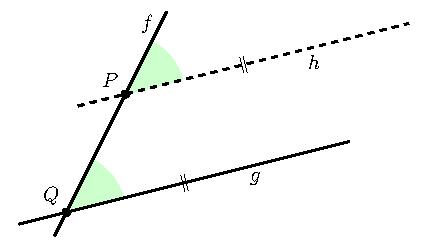
\includegraphics[width=0.5\linewidth, keepaspectratio]{figures/geometry-6.pdf}
    \caption{TODO}
    \label{fig:bild-6}
\end{figure}

\begin{beweis}
    Sei $f \in G$ mit $P \in f$. Ist $f \cap g = \emptyset$, so setze
    $h := f$. Andernfalls sei $\Set{Q} : = f \cap g$.

    Sei $\varphi$ \underline{die} Isometrie mit $\varphi(Q) = P$,
    $\varphi(P) = P'$, die die Halbebenen bzgl. $f$ nicht vertauscht.
    
    Setze $h := \varphi(g)$.

    \underline{Z.~Z.:} $h \cap g = \emptyset$.

    Andernfalls sei $\Set{R} = h \cap g$.

    \begin{figure}[htp]
        \centering
        %\documentclass[varwidth=true, border=2pt]{standalone}
\usepackage{tkz-euclide}

\begin{document}
\usetkzobj{all}
\begin{tikzpicture}
    \tkzSetUpPoint[shape=circle,size=10,color=black,fill=black]
    \tkzSetUpLine[line width=1]
    \tkzDefPoints{0/0/Q, 2/0/P, 1/2/R}


    \pgfmathsetmacro{\firstAngle}{0}
    \pgfmathsetmacro{\secondAngle}{-120}
    \path[draw,red, fill=red!40] (Q) -- ++(\firstAngle:.4) arc[start angle=\firstAngle, delta angle=\secondAngle,radius=.4];

    \tkzMarkAngle[arc=l,size=0.8cm,color=green,fill=green!20](Q,R,P)
    \path[draw] ++(-50:.2) node[rotate=-50] {$\alpha$};
    \node at (1,1.5) {$\beta$};
    \tkzDrawLine(Q,P)
    \tkzDrawLine(Q,R)
    \tkzDrawLine(P,R)
    \tkzDrawPoints(P,Q,R)
    \tkzLabelPoint[below left](P){$P$}
    \tkzLabelPoint[above left](Q){$Q$}
    \tkzLabelPoint[above=0.2cm](R){$R$}
\end{tikzpicture}
\end{document}

        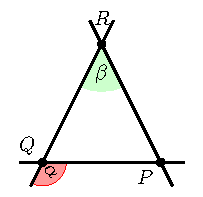
\includegraphics[width=0.5\linewidth, keepaspectratio]{figures/geometry-7.pdf}
        \caption{TODO}
        \label{fig:bild-6}
    \end{figure}
\end{beweis}

\begin{bemerkung}
    Jder Innenwinkel eines Dreiecks ist kleiner als alle nicht-anliegenden
    Außenwinkel.
\end{bemerkung}
